\documentclass{article}
\usepackage[margin=0.5in]{geometry}
\usepackage{framed}
\usepackage{graphicx}
\usepackage{wrapfig}
\usepackage{listings}
\usepackage{amsmath, esint}
\usepackage{hyperref}
\usepackage{pdfpages}
\usepackage[parfill]{parskip}
\usepackage{xcolor}
\hypersetup{
    colorlinks,
    linkcolor={red!50!black},
    citecolor={blue!50!black},
    urlcolor={blue!80!black}
}


\setlength{\parindent}{0cm}
\thispagestyle{empty}
\pagestyle{empty}
\newcommand{\Lagr}{\mathcal{L}}
\newcommand{\AnsLine}{\hspace{0.2 cm} \underline{\hspace{2 cm}}}
\newcommand{\Hgap}{\hspace{0.5cm}}
\newcommand{\Ihat}{\hat{i}}
\newcommand{\Jhat}{\hat{j}}
\newcommand{\Khat}{\hat{k}}
\newcommand{\Xhat}{\hat{x}}
\newcommand{\Yhat}{\hat{y}}
\newcommand{\Zhat}{\hat{z}}
\newcommand{\Nhat}{\hat{n}}
\newcommand{\DEL}{\vec{\nabla}}

\newcommand{\bfemph}[1]{\textbf{\emph{#1}}}

\setlength\parindent{0pt}
\def\changemargin#1#2{\list{}{\rightmargin#2\leftmargin#1}\item[]}
\let\endchangemargin=\endlist 

\title{\textbf{cMag:} A \emph{C} Version of the CLAS12 magnetic field package}

\author{D. Heddle  \\
	\emph{Christopher Newport University}  \\
         \emph{david.heddle@cnu.edu}\\
	}

\date{\today}

\begin{document}

\maketitle
\begin{abstract}
   The standard CLAS12 magnetic field package that reads and interpolates the binary field maps for the solenoid and torus was written in JAVA. The package described here reproduces the same functionality in \emph{C}. That's  \emph{C}, not \emph{C++}, 
\footnote{The reason should be obvious. \emph{C} is the most beautiful programming language ever created while, remarkably, \emph{C++} is the most hideous. This is not a matter of opinion.\\},\footnote{Pointer arithmetic, fine-grained and absolute control over memory (what could go wrong?), a preprocessor that allows you to hide critical code in impenetrable macros, and a type-unsafe compiler that looks at your line of code that equates an integer pointer to an array of strings and says: \textit{``Cool, that works for me! I'm sure you know what you are doing."} I mean, how can you not love it!\\}
 but of course it can used in a \emph{C++} program. The most important feature is that it reads the same field map files as the JAVA version. The code has been tested on OSX 10.15.4, ubuntu linux 20.04, and one other operating system. \footnote[666]{That would be Windows 10.}


\end{abstract}
\newpage

\tableofcontents
\newpage

\section {Introduction}
The magnetic field package used by \textit{ced} and by the CLAS12 reconstruction was written in JAVA. The  binary field map files used by the magnetic field package were written in JAVA\footnote{That's relevant, because JAVA sensibly decreed that data be stored in network format (which is big endian byte ordering) on all platforms independent of architecture, while most of the machines we use in CLAS are little endian.\\}. However, the CLAS12 simulation, GEMC, is written in \textit{C++} and reads ascii field map files. In spite of great effort and testing, there is always a nagging suspicion that the simulation and reconstruction are using slightly different fields. This package, \textit{cMag}, was commissioned to solve that problem, so that GEMC could read the binary maps. However, \textit{cMag} goes beyond simply reading the maps, it also provides the same tri-linear interpolation access to the fields that the JAVA package uses. This may be of use to other \textit{C} and \textit{C++} CLAS12 developments. 

\section {Where do I get it?}
\subsection {The Code}
Like everything else that isn't available on \textit{Amazon}, the \textit{cMag} distribution is available on github at:

\url{https://github.com/heddle/cmag}.

\subsection {The Field Maps}
An exception to the rule stated above, the field maps are not available on either \textit{Amazon} or github. The field map files are not part of the \texttt{cMag} distribution \footnote{This is because some people are overly sensitive about having gigabytes of field map data stored in every CLAS12-related repository.\\}. They can be downloaded from here:\

 \url{https://clasweb.jlab.org/clas12offline/magfield/}.

In Appendix B of this document you will find a description of the format of the field map files.


\section {Building}
After cloning the \textit{cMag} repository, simply work your way down to the \texttt{src} folder where you will find a \texttt{Makefile}. Now, I have not written a makefile since CLAS was a 6\ GeV toddler, but I do seem to recall that they are always very portable and never cause any grief. So I am comfortable that simply typing:

\textbf{\texttt{\$make}}

will work on any platform. 

If it worked, you should now have top-level \texttt{bin} and \texttt{lib} directories. Inside of \texttt{bin} should be an executable, \texttt{cMagTest}. Inside of \texttt{lib} should be the static library, \texttt {libcMag.a}. Use that library, and the include files in the \texttt{includes} directory, to add the \text{cMag} functionality to your program.


\subsection {Unit Testing}
Assuming the build worked (and why shouldn't it?) the first thing you should do is run \texttt{bin/cMagTest} and see if it produces happy output (it does unit testing.) 

But wait just a moment. Running  \texttt{cMagTest} is the \textit{first} thing you should do, which every programmer knows is the second thing you should do. The \textit{zeroth} thing you should do, obviously first, i.e., before the first thing, is to make sure you have bonafide CLAS12 magnetic fields.  As mentioned earlier, they can be downloaded from here:\\

 \url{https://clasweb.jlab.org/clas12offline/magfield/}.\\
\vspace{1mm}\\
Of the magnetic fields you will find there, the two that \texttt{cMagTest}  requires to run its tests are:\\

\begin{verbatim}
    Symm_solenoid_r601_phi1_z1201_13June2018.dat

    Symm_torus_r2501_phi16_z251_24Apr2018.dat
\end{verbatim} 
\vspace{1.5mm}

While the field map data directory is not hardwired into \texttt{cMagTest} (more about that anon) these two fields it tests itself upon are. 

Let's suppose your username is \texttt{yomama} and you have downloaded the magnetic fields (including but not limited to the two maps mentioned above) to the directory \texttt{/Users/yomama/data/fieldmaps}. You pass that information to \texttt{cMagTest} as the one and only command line argument it processes. That is, you type:

\textbf{\texttt{\$cMagTest /Users/yomama/data/fieldmaps}}

If you do not provide a directory as a command line argument, \texttt{cMagTest} will try one and only one place: \texttt{\$(HOME)/magfield}. So you can put the field map files there and dispense with the command line argument.

While running, \texttt{cMagTest}  will produce a \textit{lot} of output which you may or may not find interesting.  What you really care about is that \texttt{cMagTest} terminates\footnote{Depending on the OS, it may be the last line of output or the penultimate line, the latter being the case when the OS obligingly prints:\\ \texttt{Process finished with exit code 0}.\\} with the console print: 

\texttt{Program ran successfully. }

If one of the unit test fails it will say, well, something else, depending on which test failed first.
\section {Usage}
Assuming the build worked, and the testing was successful, you are ready to use the package. We will not discuss how to link \texttt{/lib/libMag.a}; you surely know how. We will discuss how to \textit{use} it after it has been successfully  linked. Here we describe only the ``public" functions, i.e. the ones you will likely use. \footnote{Of course \textit{C}, being a highly democratic and progressive language, does not hide anything, so there is really no elitist distinction between ``public" and ``private".  In \textit{C} such "binary" adjectives are discouraged.  In short, there are many more functions available, the functions that the``public" functions call upon. These functions  are accessible if you seek to cause mischief.\\} The complete API is provided in Appendix A.

We will begin with the first step, the initialization, which is the step that will most often go wrong. If you make it through the initialization, everything else should be smooth sailing.
\subsection{Initialization}

Initialization involves successfully converting the location of the field map files (their paths) into  \texttt{MagneticFieldPtr} objects, presumably one for the CLAS12 torus, and one for the CLAS12 solenoid. Once you have the valid pointers you have everything. In particular you can then ask for the field at any location.

Below we will assume that you are initializing one torus field and one solenoid field. You do not have to initialize both; if you just need one or the other then initialize just one or the other. \footnote{In fact, you could initialize two tori and three solenoids. And you do not have to initialize \textit{any} fields, but in that case we would have to wonder why you bothered to link \texttt{/libMag.a.\\}}. 

This would be a typical initialization code snippet:

\begin{verbatim} 
MagneticFieldPtr torus = initializeTorus(torusPath);
MagneticFieldPtr solenoid = initializeSolenoid(solenoidPath);

if (torus == NULL}  {
    //do something to handle a failure
}
if (solenoid == NULL}  {
    //do something to handle a failure
}

\end{verbatim}

where \texttt{torusPath} and \texttt{solenoidPath} are strings, each containing the full path to the maps you want to load. Or maybe not. It is permissible to pass \texttt{NULL} as the path argument. More about that is a second. 

How do you know it it worked? Well, there  should be some error prints if an initialization failed. But the programmatic test is whether the returned points are \texttt{NULL}. 

Don't even ask what happens if you give \texttt{initializeTorus} a solenoid map, and \texttt{initializeSolenoid}  a torus map. \footnote{Okay, since you didn't ask, I'll tell you. It's really bad. If you mismatch the calls, the secure CLAS password that we have used since the previous millennium for everything critical will be changed to \textbf{\texttt{äçäĐ™ǧẌÆ}} and nothing will work again. Ever. Okay really, nothing will happen except clarity will be sacrificed. The functions \texttt{initializeTorus} and \texttt{initializeSolenoid} are just wrappers to a single function that reads a field map. So all you will have achieved is obfuscation, which may have been your intent.\\}

Another indication that it worked is that \texttt{cMag} will print out a summary of each field that was initialized. You should look for those summaries. For example, here is a summary of the solenoid:
\footnote{The delta of $\infty$ for the $\phi$ grid of the solenoid field is a feature, not a bug.\\}

\begin{verbatim} 
========================================
SOLENOID: [/Users/heddle/magfield/Symm_solenoid_r601_phi1_z1201_13June2018.dat]
Created: Wed Jun 13 11:28:25 2018

Symmetric: true
scale factor: 1.00  
phi min:    0.0  max:  360.0  Np:    1  delta:    inf
rho min:    0.0  max:  300.0  Np:  601  delta:    0.5
  z min: -300.0  max:  300.0  Np: 1201  delta:    0.5
num field values: 721801
grid cs: cylindrical
field cs: cylindrical
length unit: cylindrical
angular unit: degrees
field unit: kG
max field at index: 102625
max field magnitude: 65.832903  kG
max field vector(0.00000  , -7.56064 , 65.39731 ), magnitude:     65.83290
max field location (phi, rho, z) = (0.00  , 42.50 , -30.00)
avg field magnitude: 3.082540   kG
\end{verbatim}

\subsubsection{Environment Variables}
So, what's this about passing \texttt{NULL} for a path to the initialization functions? In that case the initialization will reluctantly turn to environment variables: \texttt{initializeTorus}  will first try a path obtained from the environment variable \texttt{COAT\_MAGFIELD\_TORUSMAP}. If that fails, it will try \texttt{TORUSMAP}. If that fails, it will give up the ghost, as far as initializing the torus is concerned. Similarly \texttt{initializeSolenoid} will first try the environment variable \texttt{COAT\_MAGFIELD\_SOLENOIDMAP}. If that fails, it will try \texttt{SOLENOIDMAP}. 

\subsection{Settings}
How much control does the user have over what's happening under the hood? Not much. One global (i.e., it applies to all fields) option that is available is the \textit{algorithm} (for obtaining field values) setting. The user can set it to \texttt{INTERPOLATION} or \texttt{NEAREST\_NEIGHBOR}. The default is \texttt{INTERPOLATION}. 

We don't think there is ever a need to switch it to \texttt{NEAREST\_NEIGHBOR}, but should you want to, just call:

\texttt{setAlgorithm(NEAREST\_NEIGHBOR)}. 

After you get bored with that, set it back via: 

\texttt{setAlgorithm(INTERPOLATION)}.

As for field-by-field  settting, each magnetic field has a \texttt{scale}, which defaults to\ 1. And each magnetic field has ``misplacement" shifts \texttt{shiftX}, \texttt{shiftY}, and \texttt{shiftZ}, each of which defaults to 0 (units are cm). Thus you may want to do something immediate such as:
 \begin{verbatim} 
torusField->scale = -1;
\end{verbatim}
Since that is often the case. \footnote{We agonized over whether to make the default torus scaling -1, and finally chose the option we believe is most consistent with the \textit{C} zeitgeist.\\}


\subsection{Obtaining Field Values}
Here we are: the meat and potatoes section. Everything has built with nary a glitch, all the unit tests have passed,  and the field map files are downloaded, and the library \texttt{libCMag.a} is linked in. \footnote{Again, we will not comment on the link process, which for complex codes (not \texttt{cMag} which is embarrassingly simple, but for whatever is attempting to link \texttt{libCMag.a}, --which is likely to be complex beyond our ability to comprehend) generally leads to much weeping and gnashing of teeth. But just one note: \texttt{libCMag.a} does depend on the ubiquitous \textit{C} math library, \texttt{libm.a}. No doubt your code already links that with a dash of \texttt{-lm}, but for full disclosure we are putting the dependency down on paper.\\}

\subsection {Miscellany}
\subsubsection{Seeing is Believing}
I don't know about you, but I don't believe anything works unless I see it. So \texttt{cMag} comes with the ability to make an SVG image.\footnote{It was an easy choice to go SVG rather than jpeg or png or some other format.  SVG files are xml, so producing them is simply writing text files, rather than adding jpeg or png libraries that will result in you build procedure being a house O' cards. In addition, someone else already wrote exactly the minimal SVG code thet we need, in \textit{C} available at \url{https://github.com/CodeDrome/svg-library-c}. Game, set, match, point.  Okay, it's not all good news, the svg files are huge, but I don't care.}
\subsubsection{Make a Date}
In case you'd like to know how the formatted creation date is obtained from the high and low words in the header, it's like this:
\begin{verbatim}
static char *getCreationDate(FieldMapHeaderPtr headerPtr) {
     int high = headerPtr->cdHigh;
     int low = headerPtr->cdLow;

//the divide by 1000 below is because the JAVA creation time 
//(which was used in creating the maps) is in nS.

    long dlow = low & 0x00000000ffffffffL;
    time_t utime = (((long) high << 32) | (dlow & 0xffffffffL)) / 1000;
return ctime(&utime);

\end{verbatim}

\newpage
\appendix
\section{Programmer's API}
\newpage
\section{Field Map File Format}
Provided mostly for completeness, and demonstrating the raw power of \LaTeX, the fieldmap file format document has been inserted starting on the next page. If that doesn't work, the document is also included in the  \texttt{docs} directory of the \textit{cMag} distribution. \footnote{ As, self-rerentially, this document is, referring to the location where it is stored at the location where it is stored.}
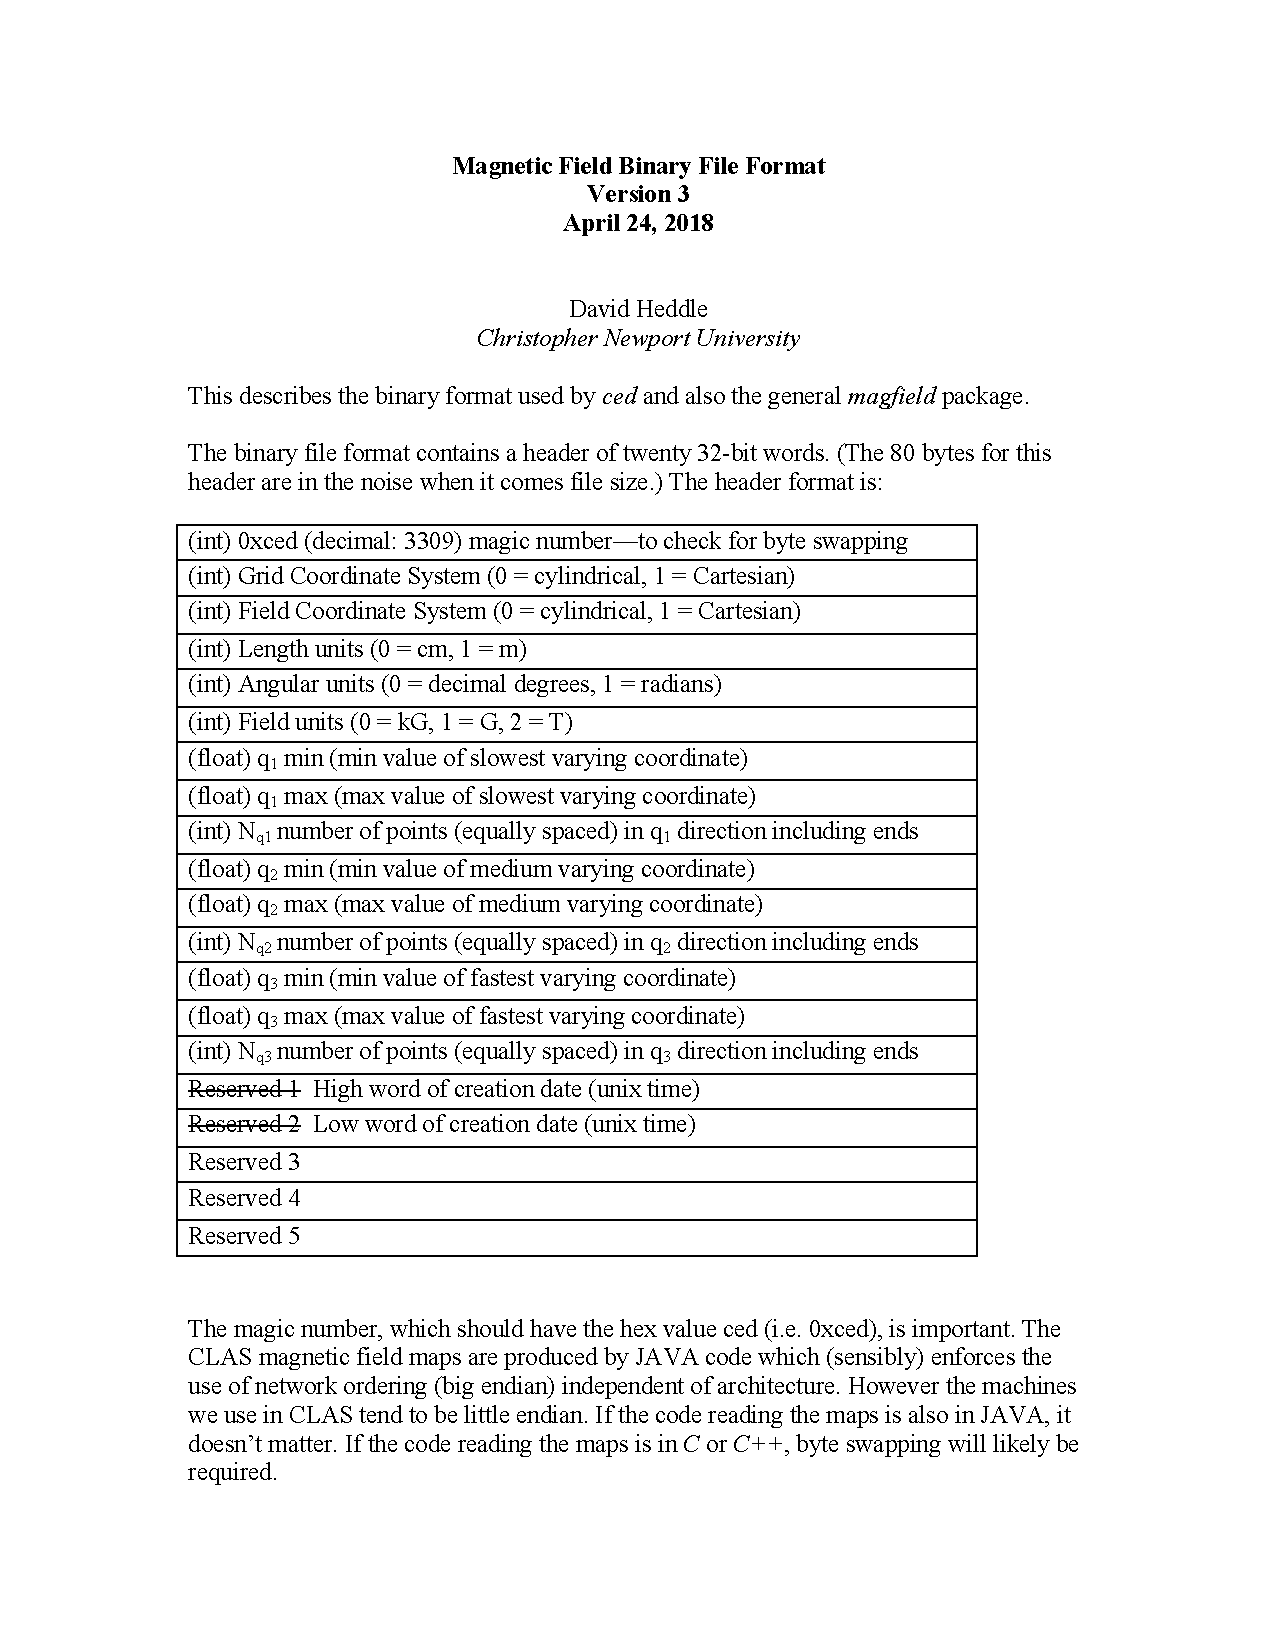
\includepdf[pages=-,pagecommand={},width=\textwidth]{FieldmapFileFormat.pdf}

------------------\\
END OF DOCUMENT
\end{document}
